\documentclass[notes,11pt, aspectratio=169]{beamer}

\usepackage{pgfpages}
\setbeameroption{hide notes}

\usepackage{helvet}
\usepackage[default]{lato}
\usepackage{array}
\usepackage{tgbonum}

\usepackage{tikz}
\usepackage{verbatim}
\setbeamertemplate{note page}{\pagecolor{yellow!5}\insertnote}
\usetikzlibrary{positioning}
\usetikzlibrary{calc}
\usetikzlibrary{arrows}
\usetikzlibrary{arrows.meta}
\usetikzlibrary{decorations.markings}
\usetikzlibrary{decorations.pathreplacing}
\usetikzlibrary{shapes.misc}
\usetikzlibrary{shapes.geometric}
\usetikzlibrary{matrix,shapes,arrows,fit,tikzmark}
\usepackage{amsmath}
\usepackage{amssymb}
\usepackage{mathtools}
\usepackage{bm}
\usepackage{mathpazo}
\usepackage{hyperref}
%\usepackage{lipsum}
%\usepackage{multimedia}
\usepackage{graphicx}
\usepackage{multirow}
\usepackage{dcolumn}
%\usepackage{bbm}   % PK-only fonts; not renderable by tectonic (indicator uses \mathbf{1})
\usepackage{pgfplots}
\pgfplotsset{compat=1.18}
\usepackage{listings}
\newcolumntype{d}[0]{D{.}{.}{5}}

\usepackage{changepage}
\usepackage{appendixnumberbeamer}
\newcommand{\beginbackup}{
   \newcounter{framenumbervorappendix}
   \setcounter{framenumbervorappendix}{\value{framenumber}}
   \setbeamertemplate{footline}
   {
     \leavevmode%
     \hline
     box{%
       \begin{beamercolorbox}[wd=\paperwidth,ht=2.25ex,dp=1ex,right]{footlinecolor}%
       \end{beamercolorbox}}%
     \vskip0pt%
   }
 }
\newcommand{\backupend}{
   \addtocounter{framenumbervorappendix}{-\value{framenumber}}
   \addtocounter{framenumber}{\value{framenumbervorappendix}}
}

\usepackage[space]{grffile}
\usepackage{booktabs}
\newcommand\independent{\protect\mathpalette{\protect\independenT}{\perp}}
\def\independenT#1#2{\mathrel{\rlap{$#1#2$}\mkern2mu{#1#2}}}
\DeclareMathOperator{\Supp}{Supp}
\DeclareMathOperator*{\argmin}{arg\,min}
\DeclareMathOperator{\trace}{trace}

\definecolor{blue}{RGB}{0,114,178}
\definecolor{red}{RGB}{213,94,0}
\definecolor{yellow}{RGB}{240,228,66}
\definecolor{green}{RGB}{0,158,115}

\hypersetup{
  colorlinks=true,
  linkbordercolor = {white},
  linkcolor = {blue}
}

\definecolor{MyBackground}{RGB}{255,253,218}

\newenvironment{transitionframe}{
  \setbeamercolor{background canvas}{bg=yellow}
  \begin{frame}}{
    \end{frame}
}

\setbeamercolor{frametitle}{fg=blue}
\setbeamercolor{title}{fg=black}
\setbeamertemplate{footline}[frame number]
\setbeamertemplate{navigation symbols}{}
\setbeamertemplate{itemize items}{-}
\setbeamercolor{itemize item}{fg=blue}
\setbeamercolor{itemize subitem}{fg=blue}
\setbeamercolor{enumerate item}{fg=blue}
\setbeamercolor{enumerate subitem}{fg=blue}
\setbeamercolor{button}{bg=MyBackground,fg=blue,}

\setbeamercolor{section in toc}{fg=blue}
\setbeamercolor{subsection in toc}{fg=red}
\setbeamersize{text margin left=1em,text margin right=1em}

\newenvironment{wideitemize}{\itemize\addtolength{\itemsep}{10pt}}{\enditemize}

\lstset{
    language=Python,
    basicstyle=\ttfamily\scriptsize,
    keywordstyle=\color{blue}\bfseries,
    stringstyle=\color{red!70!black},
    commentstyle=\color{green!50!black}\itshape,
    numbers=left,
    numberstyle=\tiny\color{gray},
    numbersep=5pt,
    frame=single,
    breaklines=true,
    backgroundcolor=\color{gray!5},
    showstringspaces=false,
    tabsize=4
}

\newcommand{\vx}{\mathbf{x}}
\newcommand{\vw}{\mathbf{w}}
\newcommand{\vy}{\mathbf{y}}
\newcommand{\vu}{\mathbf{u}}
\newcommand{\vv}{\mathbf{v}}
\newcommand{\vA}{\mathbf{A}}
\newcommand{\vB}{\mathbf{B}}
\newcommand{\vz}{\mathbf{z}}
\newcommand{\vU}{\mathbf{U}}
\newcommand{\vV}{\mathbf{V}}
\newcommand{\vW}{\mathbf{W}}
\newcommand{\vX}{\mathbf{X}}
\newcommand{\vY}{\mathbf{Y}}
\newcommand{\vSigma}{\boldsymbol{\Sigma}}
\newcommand{\vLambda}{\boldsymbol{\Lambda}}
\newcommand{\R}{\mathbb{R}}
\newcommand{\E}{\mathbb{E}}
\newcommand{\Frob}{\mathrm{Fro}}


\title[]{\textcolor{blue}{Machine Learning II}\\ \textcolor{black}{\normalsize Lecture 4: Matrix Factorization and Latent Factors}}
\author[Quispe]{}
\institute[ENEI]{\small{Alexander Quispe \\ ENEI -- INEI \,\textperiodcentered\, PEU-CD 2026}}
\date{October 16, 2026}


\begin{document}

\begin{frame}[plain]\titlepage\end{frame}

\begin{frame}{Outline}\tableofcontents\end{frame}


\tikzset{
        every picture/.style={remember picture,baseline},
        every node/.style={anchor=base,align=center,outer sep=1.5pt},
        every path/.style={thick},
        }
\tikzstyle{every picture}+=[remember picture]
\tikzstyle{mybox} =[draw=black, very thick, rectangle, inner sep=10pt, inner ysep=20pt]
\tikzstyle{fancytitle} =[draw=black,fill=red, text=white]




% ============================================================
\section{Recap and Motivation}
% ============================================================

\begin{transitionframe}
\begin{center}
{\Huge \textbf{Recap \& Motivation}}\\[10pt]
{\large From sequences to structure}
\end{center}
\end{transitionframe}

\begin{frame}
\frametitle{Where We've Been}

\textbf{Lectures 1--5 covered \emph{supervised} learning with deep models:}
\begin{itemize}
    \item Lecture 1: perceptrons, the universal approximation theorem.
    \item Lecture 2: backpropagation.
    \item Lecture 3: regularization, SGD.
    \item Lecture 4: convolutional networks.
    \item Lecture 5: recurrent networks (RNN, LSTM, GRU).
\end{itemize}

\vspace{6pt}
\textbf{Common pattern:} we always had labeled pairs $(\vx_i, y_i)$ and minimized a prediction loss.

\vspace{8pt}
\textcolor{red}{Today we shift gears: what if we have only the matrix $\vY$, with no separate features and many missing entries?}
\end{frame}

\begin{frame}
\frametitle{Three Motivating Problems}

\begin{enumerate}
    \item \textcolor{blue}{\textbf{Recommendation:}} a matrix of user-by-item ratings, mostly empty. Predict the missing entries.

    \vspace{6pt}
    \item \textcolor{blue}{\textbf{Causal panels:}} a matrix of unit-by-time outcomes, where treated units have unobserved counterfactuals. Recover what would have happened without treatment.

    \vspace{6pt}
    \item \textcolor{blue}{\textbf{Topic discovery:}} a document-by-word count matrix. Find a small set of topics that explain the documents.
\end{enumerate}

\vspace{12pt}
\begin{tikzpicture}
\node [mybox] (box){%
    \begin{minipage}{0.93\textwidth}
    \vspace{-4pt}
    All three are \textbf{matrix factorization} problems:
    \[
        \vY \approx \vU \vV^\top
    \]
    with $\vU$ low-rank rows and $\vV$ low-rank columns.
    \end{minipage}
};
\node[fancytitle, right=10pt] at (box.north west) {Today's unifying view};
\end{tikzpicture}
\end{frame}

\begin{frame}
\frametitle{Why a Deep Learning Class Cares}

\textbf{Three reasons to spend a class on this:}

\vspace{6pt}
\begin{enumerate}
    \item \textbf{Embedding layers are matrix factorization.} \texttt{nn.Embedding(N, K)} stores one row per entity. The dot product of two rows is exactly $\vu_i^\top \vv_j$.

    \vspace{6pt}
    \item \textbf{PCA is a linear autoencoder.} Replacing the linear bottleneck with a neural network gives you a deep autoencoder.

    \vspace{6pt}
    \item \textbf{Word2vec is implicit matrix factorization.} The skip-gram with negative-sampling objective factorizes a shifted PMI matrix (Levy \& Goldberg, 2014).
\end{enumerate}

\vspace{8pt}
\textcolor{red}{Latent factor models are the linear ancestor of every modern embedding-based model.}
\end{frame}

\begin{frame}
\frametitle{Today's Roadmap (Annotated)}

\begin{enumerate}
    \item \textbf{Linear algebra recap.} Orthogonal matrices, SVD, PCA -- the foundation.
    \item \textbf{Matrix norms.} Frobenius and trace norms; the convex relaxation of rank.
    \item \textbf{Latent factor models.} Collaborative filtering, missing values, alternating optimization. \textcolor{red}{Reframed as panel data with missing potential outcomes.}
    \item \textbf{Multitask learning.} Latent factors as shared low-dimensional features across tasks.
    \item \textbf{Non-negative matrix factorization.} Parts-based representations, topic modeling.
    \item \textbf{Bridge to deep learning.} Embedding layers, autoencoders, word2vec.
\end{enumerate}
\end{frame}
% ============================================================



% ----------------------------------------------------------------------
% NEW: why is U a rotation? (chain of reasoning)
% ----------------------------------------------------------------------

% ----------------------------------------------------------------------
% NEW: reading theta off the matrix entries
% ----------------------------------------------------------------------

% ----------------------------------------------------------------------
% NEW: rotation vs reflection
% ----------------------------------------------------------------------

% ----------------------------------------------------------------------
% NEW: 3D rotations
% ----------------------------------------------------------------------


% ----------------------------------------------------------------------
% NEW: shapes / dimensions of the projection
% ----------------------------------------------------------------------

% ----------------------------------------------------------------------
% NEW: worked example
% ----------------------------------------------------------------------

% ----------------------------------------------------------------------
% NEW: Pythagoras
% ----------------------------------------------------------------------



% ----------------------------------------------------------------------
% NEW: "Centering the data" -- precondition for everything below
% ----------------------------------------------------------------------




\begin{frame}{What We Carry Over From Machine Learning I}\small
Lecture 6 of ML I proved, in full, the linear-algebra facts this lecture builds on. They are used, not re-derived:
\begin{itemize}
  \item \textbf{Projections.} $\mathbf{P}=\mathbf{V}\mathbf{V}^\top$ with $\mathbf{V}^\top\mathbf{V}=\mathbf{I}_k$ is symmetric and idempotent; $\|\mathbf{x}\|^2=\|\mathbf{P}\mathbf{x}\|^2+\|(\mathbf{I}-\mathbf{P})\mathbf{x}\|^2$.
  \item \textbf{PCA.} The top eigenvector of $\mathbf{S}=\tfrac1N\mathbf{X}^\top\mathbf{X}$ maximizes projected variance (Lagrangian); the top $k$ maximize $\operatorname{tr}(\mathbf{V}^\top\mathbf{S}\mathbf{V})$ (Ky Fan); retained variance $=\lambda_1+\dots+\lambda_k$; maximum variance $\Leftrightarrow$ minimum reconstruction error.
  \item \textbf{SVD.} For centred $\mathbf{X}=\mathbf{U}\mathbf{D}\mathbf{V}^\top$, the right singular vectors are the principal components and $\lambda_j=d_j^2/N$.
  \item \textbf{Eckart--Young.} Among all matrices of rank $\le k$, the truncated SVD $\mathbf{U}_k\mathbf{D}_k\mathbf{V}_k^\top$ is closest to $\mathbf{X}$ in Frobenius norm, with error $\sum_{j>k}d_j^2$.
\end{itemize}
\begin{alertblock}{Today's question}
Eckart--Young needs \emph{every} entry of $\mathbf{X}$. What if most entries are missing --- a user has rated 20 of 10{,}000 films, a firm is observed only before a policy? That is the latent-factor problem, and the trace norm is how the rank constraint survives it.
\end{alertblock}
\end{frame}


% ============================================================
\section{Matrix Norms}
% ============================================================

\begin{transitionframe}
\begin{center}
{\Huge \textbf{Matrix Norms}}\\[10pt]
{\large Frobenius, trace, and the rank surrogate}
\end{center}
\end{transitionframe}

\begin{frame}
\frametitle{The Frobenius Norm}

\textbf{Definition:}
\[
    \|\vX\|_\Frob = \sqrt{\sum_{i,j} X_{ij}^2}
\]
the matrix version of the L2 vector norm.

\vspace{8pt}
\textbf{In terms of singular values:}
\[
    \|\vX\|_\Frob^2 = \sum_d \sigma_d^2
\]

\vspace{4pt}
\textbf{Why?} Use the trace identity $\|\vX\|_\Frob^2 = \trace(\vX^\top \vX)$ and substitute SVD:
\[
    \trace(\vX^\top \vX) = \trace(\vV \vSigma^2 \vV^\top) = \trace(\vSigma^2) = \sum_d \sigma_d^2.
\]

\vspace{6pt}
\textcolor{blue}{Useful for L2-style regularization of matrix-valued parameters.}
\end{frame}

\begin{frame}
\frametitle{The Rank Norm and the Trace Norm}

\textbf{Rank norm} (count of nonzero singular values):
\[
    \|\vX\|_{\mathrm{Rank}} = \sum_d \mathbf{1}[\sigma_d > 0]
\]

\vspace{4pt}
\textcolor{red}{Problem:} this is discrete and discontinuous -- impossible to optimize with gradient methods.

\vspace{12pt}
\textbf{Trace norm (a.k.a.\ nuclear norm):}
\[
    \|\vX\|_* = \sum_d \sigma_d = \trace\!\left(\sqrt{\vX^\top \vX}\right)
\]

\vspace{6pt}
\textbf{Intuition:} this is the L1 norm \emph{of the singular values}.

\vspace{4pt}
\textcolor{blue}{The trace norm is the convex envelope of the rank norm} -- the same way L1 is the convex relaxation of L0.
\end{frame}

\begin{frame}
\frametitle{Convex Relaxation: A Familiar Pattern}

\textbf{For vectors:}
\begin{center}
\begin{tabular}{lll}
\toprule
\textbf{Goal} & \textbf{Discrete penalty} & \textbf{Convex surrogate} \\
\midrule
sparse vector & $\|\vw\|_0$ (count of nonzeros) & $\|\vw\|_1$ \\
\bottomrule
\end{tabular}
\end{center}

\vspace{6pt}
$\Rightarrow$ Lasso regression.

\vspace{12pt}
\textbf{For matrices:}
\begin{center}
\begin{tabular}{lll}
\toprule
\textbf{Goal} & \textbf{Discrete penalty} & \textbf{Convex surrogate} \\
\midrule
low-rank matrix & $\mathrm{rank}(\vX)$ & $\|\vX\|_*$ (trace norm) \\
\bottomrule
\end{tabular}
\end{center}

\vspace{6pt}
$\Rightarrow$ \textcolor{red}{Trace-norm regularized matrix factorization.}

\vspace{12pt}
\textbf{Same idea, different object.} Both replace a non-convex sparsity penalty with its tightest convex lower bound.
\end{frame}

\begin{frame}
\frametitle{Useful Properties of Matrix Norms}

\textbf{Cauchy--Schwarz:}
\[
    \langle \vA, \vB\rangle^2 = \trace(\vA^\top \vB)^2 \leq \|\vA\|_\Frob^2 \cdot \|\vB\|_\Frob^2
\]

\vspace{4pt}
\textbf{AM--GM inequality:}
\[
    \|\vA\| \cdot \|\vB\| \leq \tfrac{1}{2}(\|\vA\|^2 + \|\vB\|^2)
\]

\vspace{4pt}
\textbf{Orthogonal invariance:} for full-rank orthogonal $\vU$,
\[
    \|\vU \vA\|_\Frob = \|\vA\|_\Frob, \qquad \|\vU \vA\|_* = \|\vA\|_*.
\]

\vspace{6pt}
\textcolor{blue}{Both norms see only singular values, not the choice of basis.}

\vspace{6pt}
\textbf{Trace norm of a diagonal matrix:} just the L1 of its diagonal entries:
\[
    \|\vA\|_* = \sum_i |A_{ii}| \quad\text{if } \vA \text{ is square diagonal.}
\]
\end{frame}


% ============================================================
\section{Latent Factor Models}
% ============================================================

\begin{transitionframe}
\begin{center}
{\Huge \textbf{Latent Factor Models}}\\[10pt]
{\large Low-rank reasoning with missing data}
\end{center}
\end{transitionframe}

\begin{frame}
\frametitle{Motivation: The Netflix Problem}

\textbf{Setup:} an $M \times N$ matrix $\vY$ where $Y_{ij}$ is the rating user $i$ gave movie $j$.

\vspace{6pt}
\textbf{Goal:} predict the ratings users \emph{didn't} provide.

\vspace{8pt}
\begin{center}
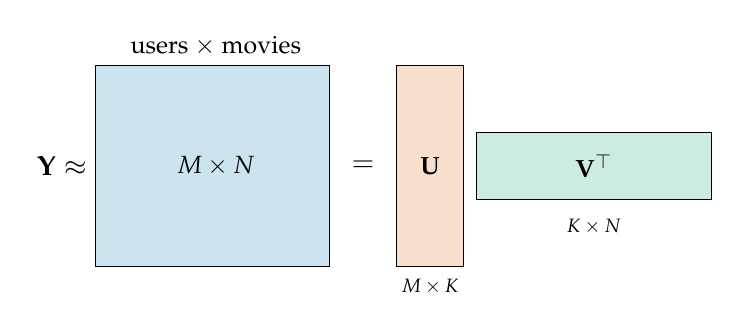
\begin{tikzpicture}[scale=0.85]
    \node at (-3, 0) {$\vY \approx$};
    \draw[fill=blue!20] (-2.5, -1.5) rectangle (1, 1.5);
    \node at (-0.7, 0) {\small $M \times N$};
    \node[above] at (-0.7, 1.5) {\small users $\times$ movies};

    \node at (1.5, 0) {$=$};

    \draw[fill=red!20] (2, -1.5) rectangle (3, 1.5);
    \node at (2.5, 0) {\small $\vU$};
    \node at (2.5, -1.8) {\scriptsize $M \times K$};

    \draw[fill=green!20] (3.2, -0.5) rectangle (6.7, 0.5);
    \node at (4.95, 0) {\small $\vV^\top$};
    \node at (4.95, -0.9) {\scriptsize $K \times N$};
\end{tikzpicture}
\end{center}

\vspace{8pt}
\textbf{Model:}
\[
    Y_{ij} \approx \vu_i^\top \vv_j
\]
where $\vu_i$ is a $K$-dimensional ``user vector'' and $\vv_j$ is a ``movie vector''. The $K$ \textcolor{red}{latent factors} encode taste and content.

\vspace{4pt}
\textbf{If $\vY$ were complete, we'd just take its SVD.} But it isn't.
\end{frame}

% ----------------------------------------------------------------------
% NEW: worked numerical example, part 1 -- setup
% ----------------------------------------------------------------------
\begin{frame}
\frametitle{Worked example: $4$ users, $5$ movies, $K=2$}

\textbf{Observed ratings} ($-2$ to $+2$ scale; $?$ = missing):
{\small
\[
\vY \;=\;
\begin{array}{r|ccccc}
        & \text{Aveng.} & \text{Schind.} & \text{Sav.Ry.} & \text{Nott.Hill} & \text{Dune} \\\hline
\text{Alice} & +1.6 & -1.6 & ? & ? & +0.6 \\
\text{Bob}   & -1.1 & ?    & +0.3 & -0.1 & ? \\
\text{Carol} & ?    & -0.4 & +1.1 & ?    & +1.0 \\
\text{Dave}  & -0.2 & ?    & ?    & +1.0 & -0.9
\end{array}
\]
}
$M\!=\!4$, $N\!=\!5$, $11$ of $20$ entries observed.

\vspace{6pt}
\textbf{After fitting,} one possible solution is
{\small
\[
\vU = \begin{pmatrix}
+1.0 & +0.8 \\
-0.5 & -0.7 \\
+0.9 & -0.6 \\
-0.7 & +0.6
\end{pmatrix}_{\!\!4\times 2}
\qquad
\vV = \begin{pmatrix}
+1.0 & +0.8 \\
-1.0 & -0.8 \\
+0.6 & -0.9 \\
-0.8 & +0.7 \\
+0.9 & -0.4
\end{pmatrix}_{\!\!5\times 2}
\]
}
Rows of $\vU$ = user vectors $\vu_i$; rows of $\vV$ = movie vectors $\vv_j$. The two latent dimensions happen to align with \emph{action--ness} (col.\ 1) and \emph{lightness} (col.\ 2) --- labels are read off \emph{post hoc}.
\end{frame}

% ----------------------------------------------------------------------
% NEW: worked numerical example, part 2 -- predictions
% ----------------------------------------------------------------------
\begin{frame}
\frametitle{Worked example: predictions $\hat{\vY} = \vU \vV^\top$}

\textbf{Recipe:} $\hat Y_{ij} = \vu_i^\top \vv_j$.

\vspace{4pt}
\textbf{Observed entry} --- Alice $\times$ Avengers:
\[
    \vu_{\text{Alice}}^\top \vv_{\text{Aveng.}}
    = (1.0)(1.0) + (0.8)(0.8) = 1.00 + 0.64 = 1.64.
\]
Observed: $+1.6$. \checkmark

\vspace{4pt}
\textbf{Missing entry} --- Alice $\times$ Saving Ryan:
\[
    \vu_{\text{Alice}}^\top \vv_{\text{Sav.Ry.}}
    = (1.0)(0.6) + (0.8)(-0.9) = 0.60 - 0.72 = -0.12.
\]
Action match cancels with tone mismatch $\Rightarrow$ Alice would skip it.

\vspace{4pt}
\textbf{Full $\vU\vV^\top$} (\textbf{bold} = was missing in $\vY$):
{\small
\[
\hat{\vY} = \begin{array}{r|ccccc}
        & \text{Aveng.} & \text{Schind.} & \text{Sav.Ry.} & \text{Nott.Hill} & \text{Dune} \\\hline
\text{Alice} & +1.64 & -1.64 & \mathbf{-0.12} & \mathbf{-0.24} & +0.58 \\
\text{Bob}   & -1.06 & \mathbf{+1.06} & +0.33 & -0.09 & \mathbf{-0.17} \\
\text{Carol} & \mathbf{+0.42} & -0.42 & +1.08 & \mathbf{-1.14} & +1.05 \\
\text{Dave}  & -0.22 & \mathbf{+0.22} & \mathbf{-0.96} & +0.98 & -0.87
\end{array}
\]
}
\textbf{Recommendations:} Bob $\to$ \emph{Schindler}; Carol $\to$ \emph{Avengers}; Dave $\to$ \emph{Notting Hill}.

\vspace{2pt}
{\footnotesize \textcolor{gray}{Caveat: $\vU\vV^\top$ is unique, but $\vU$ and $\vV$ individually are not. Replacing $\vU \to \vU\mathbf{Q}$ and $\vV \to \vV\mathbf{Q}^{-\top}$ for any invertible $\mathbf{Q}$ leaves all predictions unchanged.}}
\end{frame}

\begin{frame}
\frametitle{Latent Factors: Interpretation}

\textbf{Hypothetical 2D factor space:}

\vspace{4pt}
\begin{center}
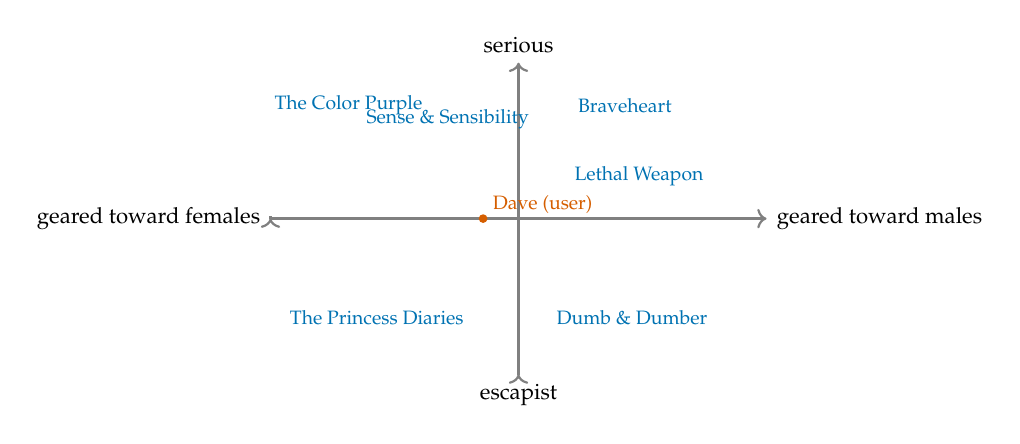
\begin{tikzpicture}[scale=0.9]
    \draw[->, thick, gray] (-3.5, 0) -- (3.5, 0) node[right, black] {\footnotesize geared toward males};
    \draw[<-, thick, gray] (-3.5, 0) -- (-3.5, 0) node[left, black] {\footnotesize geared toward females};
    \draw[->, thick, gray] (0, -2.2) -- (0, 2.2) node[above, black] {\footnotesize serious};
    \draw[<-, thick, gray] (0, -2.2) -- (0, -2.2) node[below, black] {\footnotesize escapist};

    \node[blue] at (-2.4, 1.6) {\scriptsize The Color Purple};
    \node[blue] at (-1, 1.4) {\scriptsize Sense \& Sensibility};
    \node[blue] at (1.5, 1.6) {\scriptsize Braveheart};
    \node[blue] at (1.7, 0.6) {\scriptsize Lethal Weapon};
    \node[blue] at (-2, -1.4) {\scriptsize The Princess Diaries};
    \node[blue] at (1.6, -1.4) {\scriptsize Dumb \& Dumber};

    \node[red, right] at (-0.5, 0.2) {\scriptsize Dave (user)};
    \draw[red, fill=red] (-0.5, 0) circle (1.5pt);
\end{tikzpicture}
\end{center}

\vspace{4pt}
\textbf{Reading the factors:}
\begin{itemize}
    \item Movie vector $\vv_j$ = position in factor space (e.g., serious $+$ male-skewed).
    \item User vector $\vu_i$ = the user's preference direction.
    \item Predicted rating $\vu_i^\top \vv_j$ = how aligned the user's taste is with the movie.
\end{itemize}

\textcolor{red}{Crucially, no one tells us the axes -- they emerge from the data.}
\end{frame}

\begin{frame}
\frametitle{Collaborative Filtering: The Real Problem}

\textbf{Reality:} most of $\vY$ is missing.

\vspace{6pt}
\begin{itemize}
    \item $M$ users $\times$ $N$ items, with $M, N$ in the millions.
    \item Each user rates only a tiny fraction of items.
    \item No user features, no item features -- only the observed ratings.
\end{itemize}

\vspace{8pt}
\textbf{Goal:} learn $\vU \in \R^{M \times K}$ and $\vV \in \R^{N \times K}$ such that $\vU \vV^\top$ reconstructs the observed entries \emph{and} fills in the missing ones plausibly.

\vspace{8pt}
\textbf{Assumption that makes this possible:}
\begin{tikzpicture}
\node [mybox] (box){%
    \begin{minipage}{0.93\textwidth}
    \vspace{-4pt}
    There exists a low-rank subspace ($K \ll M, N$) that captures all the variation across users and items.
    \end{minipage}
};
\node[fancytitle, right=10pt] at (box.north west) {Low-rank assumption};
\end{tikzpicture}
\end{frame}

\begin{frame}
\frametitle{Latent Factor Formulation}

\textbf{Observed entries} $S = \{(i, j) : Y_{ij} \text{ observed}\}$.

\vspace{4pt}
Let $\omega_{ij} = 1$ if $(i,j) \in S$, else 0.

\vspace{8pt}
\textbf{Objective:}
\[
    \argmin_{\vU, \vV} \;
    \frac{\lambda}{2}\!\left(\|\vU\|_\Frob^2 + \|\vV\|_\Frob^2\right)
    + \sum_{i,j} \omega_{ij}\bigl(Y_{ij} - \vu_i^\top \vv_j\bigr)^2
\]

\vspace{6pt}
\textbf{Two terms, doing different jobs:}
\begin{itemize}
    \item \textcolor{red}{Reconstruction loss}: fit observed ratings.
    \item \textcolor{blue}{Frobenius regularizer}: shrink $\vU, \vV$ toward zero. Prevents overfitting and -- as we'll see -- caps the effective rank.
\end{itemize}

\vspace{6pt}
\textbf{Hyperparameter:} $\lambda$ controls bias--variance tradeoff. Tune by held-out validation.
\end{frame}

\begin{frame}
\frametitle{Connection to the Trace Norm}

\textbf{Claim:} the Frobenius regularizer on $(\vU, \vV)$ equals a trace-norm penalty on $\vW = \vU \vV^\top$.

\vspace{6pt}
Formally,
\[
    \|\vW\|_* = \min_{\vW = \vU \vV^\top} \tfrac{1}{2}\!\left(\|\vU\|_\Frob^2 + \|\vV\|_\Frob^2\right).
\]

\vspace{8pt}
\textbf{Proof sketch (one direction):} let $\vW = \vU \vSigma \vV^\top$ be the SVD, and choose $\vA = \vU \sqrt{\vSigma}$, $\vB = \vV \sqrt{\vSigma}$. Then $\vA \vB^\top = \vW$ and
\[
    \tfrac{1}{2}(\|\vA\|_\Frob^2 + \|\vB\|_\Frob^2) = \tfrac{1}{2}(\trace(\vSigma) + \trace(\vSigma)) = \trace(\vSigma) = \|\vW\|_*.
\]

\vspace{6pt}
\textbf{Why care?} \textcolor{red}{The Frobenius regularizer on the factors is \emph{secretly} a low-rank inducer on the product.} Same effect, but easier to optimize because the factors are explicit and small.
\end{frame}

\begin{frame}
\frametitle{The Same Idea: Three Equivalent Views}

\begin{center}
\begin{tabular}{p{4.5cm} p{8cm}}
\toprule
\textbf{View} & \textbf{Penalty} \\
\midrule
Rank-constrained & rank$(\vW) \leq K$ (non-convex) \\[4pt]
Trace-norm regularized & $\lambda \|\vW\|_*$ (convex, but slow) \\[4pt]
Factorized Frobenius & $\frac{\lambda}{2}(\|\vU\|_\Frob^2 + \|\vV\|_\Frob^2)$ with $\vW = \vU \vV^\top$ (non-convex but fast) \\
\bottomrule
\end{tabular}
\end{center}

\vspace{12pt}
\textbf{In practice:} the third form wins. It's smooth, it has explicit factors we can store, and (for fixed $K$) it scales to massive matrices.

\vspace{6pt}
\textcolor{blue}{This is the form used by every recommender system, every embedding layer, and every modern matrix-completion econometrics method.}
\end{frame}


% ============================================================
% Panel data reframing -- the key MECA pivot
% ============================================================

\begin{frame}
\frametitle{This Is Just Panel Data}

\textbf{Econometrics setup} (e.g., Bai 2009, \emph{Econometrica}):
\[
    Y_{it} = \boldsymbol\lambda_i^\top \mathbf{F}_t + \varepsilon_{it}
\]
where $\boldsymbol\lambda_i$ are unit-specific ``loadings'' and $\mathbf{F}_t$ are time-specific ``factors''.

\vspace{6pt}
\textbf{Stacking:} let $\boldsymbol\Lambda \in \R^{N \times K}$ stack the loadings, $\mathbf{F} \in \R^{T \times K}$ stack the factors. Then
\[
    \vY = \boldsymbol\Lambda \mathbf{F}^\top + \boldsymbol\varepsilon.
\]

\vspace{6pt}
\textcolor{red}{This is \emph{exactly} the latent factor model with $\vU = \boldsymbol\Lambda$ and $\vV = \mathbf{F}$.}

\vspace{8pt}
\begin{tabular}{ll}
\toprule
\textbf{ML language} & \textbf{Econometrics language} \\
\midrule
user vectors $\vU$ & unit fixed effects (loadings) $\boldsymbol\Lambda$ \\
item vectors $\vV$ & time fixed effects (factors) $\mathbf{F}$ \\
low rank $K$ & limited heterogeneity \\
missing entries & untreated / treated observations \\
\bottomrule
\end{tabular}
\end{frame}

\begin{frame}
\frametitle{Causal Panel Data: The Counterfactual}

\textbf{Setup:} units $i$ over time $t$. Treatment $D_{it} \in \{0, 1\}$.

\vspace{4pt}
We observe $Y_{it}(0)$ when $D_{it} = 0$, and $Y_{it}(1)$ when $D_{it} = 1$.

\vspace{6pt}
\textbf{Causal effect of interest:}
\[
    \tau_{it} = Y_{it}(1) - Y_{it}(0).
\]

\textcolor{red}{We never observe both. But we observe one, and the other is exactly a missing matrix entry.}

\vspace{8pt}
\textbf{Idea (Athey, Bai, Imbens, Khosravi, 2021, JASA):}
\begin{enumerate}
    \item Stack $Y(0)$ for all units and time periods into a matrix.
    \item Mask the entries where $D_{it} = 1$ (missing counterfactual).
    \item Run latent-factor matrix completion on the masked matrix.
    \item Predicted entries are estimated counterfactuals; subtract from observed treated to get $\hat\tau_{it}$.
\end{enumerate}

\vspace{4pt}
\textcolor{blue}{Same algorithm as Netflix -- different application, profound implications.}
\end{frame}

\begin{frame}
\frametitle{Synthetic Control as a Special Case}

\textbf{Classical synthetic control} (Abadie et al., 2010): the counterfactual of a treated unit is a weighted average of control units.

\vspace{8pt}
\textbf{Matrix completion view:}
\begin{itemize}
    \item Restrict to one treated unit + many controls.
    \item Pre-treatment fit determines the unit's loading $\boldsymbol\lambda_i$.
    \item Time factors $\mathbf{F}_t$ come from controls.
    \item Counterfactual = $\boldsymbol\lambda_i^\top \mathbf{F}_t$.
\end{itemize}

\vspace{8pt}
\textbf{Why matrix completion is more general:}
\begin{itemize}
    \item Handles \emph{multiple} treated units.
    \item Handles staggered adoption (different units treated at different times).
    \item No simplex constraint on weights.
    \item Implements the same low-rank assumption with fewer restrictions.
\end{itemize}

\vspace{4pt}
\textbf{Software:} \texttt{gsynth} (R, Xu 2017) and \texttt{pysyncon} (Python).
\end{frame}

\begin{frame}
\frametitle{Optimization: How Do We Actually Fit This?}

\textbf{Objective:}
\[
    \mathcal{L}(\vU, \vV) = \frac{\lambda}{2}(\|\vU\|_\Frob^2 + \|\vV\|_\Frob^2) + \sum_{i,j} \omega_{ij}(Y_{ij} - \vu_i^\top \vv_j)^2
\]

\vspace{6pt}
\textbf{Bad news:} jointly non-convex in $(\vU, \vV)$.

\vspace{4pt}
\textbf{Good news:} \textcolor{red}{convex in $\vU$ if $\vV$ is fixed,} and vice versa. This suggests two strategies.

\vspace{8pt}
\textbf{Two algorithms:}
\begin{enumerate}
    \item \textbf{Stochastic gradient descent (SGD):} update one parameter at a time using a single $(i, j)$ at a time.
    \item \textbf{Alternating Least Squares (ALS):} fix $\vV$, solve for $\vU$ optimally; then fix $\vU$, solve for $\vV$.
\end{enumerate}
\end{frame}

\begin{frame}
\frametitle{ALS: Closed-Form Update}

Fix $\vV$ and ask: what is the optimal $\vu_i$ for user $i$?

\vspace{4pt}
Take $\partial \mathcal{L} / \partial \vu_i = 0$:
\[
    \lambda \vu_i \;-\; \sum_j \omega_{ij} \vv_j (Y_{ij} - \vu_i^\top \vv_j) \;=\; 0.
\]

\vspace{4pt}
Rearranging:
\[
    \boxed{\;\vu_i \;=\; \Bigl(\lambda \mathbf{I}_K + \sum_j \omega_{ij}\, \vv_j \vv_j^\top\Bigr)^{-1} \Bigl(\sum_j \omega_{ij}\, Y_{ij}\, \vv_j\Bigr)\;}
\]

\vspace{6pt}
\textbf{This is just regularized linear regression} of user $i$'s observed ratings on the (fixed) movie vectors.

\vspace{8pt}
\textbf{ALS algorithm:}
\begin{enumerate}
    \item Initialize $\vU, \vV$ randomly.
    \item Loop: for each $i$, update $\vu_i$ using the formula above. Then for each $j$, update $\vv_j$ symmetrically.
    \item Until convergence.
\end{enumerate}
\end{frame}

\begin{frame}
\frametitle{SGD vs ALS: Tradeoffs}

\renewcommand{\arraystretch}{1.3}
\begin{center}
{\small
\begin{tabular}{p{4cm} p{4.5cm} p{4.5cm}}
\toprule
\textbf{Aspect} & \textbf{ALS} & \textbf{SGD} \\
\midrule
Iterations to converge & few (10--50) & many (millions of steps) \\
Per-iteration cost & $O(K^3)$ matrix solve per row & $O(K)$ per observation \\
Parallelism & easy across rows & harder; per-step updates \\
Streaming data & no -- needs full matrix & yes -- one observation at a time \\
High dimensions ($K$ large) & slow & fast \\
\bottomrule
\end{tabular}
}
\end{center}

\vspace{8pt}
\textbf{Practical advice:}
\begin{itemize}
    \item Small to medium $K$ ($\leq 50$), data fits in memory $\to$ \textbf{ALS}.
    \item Massive data, streaming, or large $K$ $\to$ \textbf{SGD} (or its mini-batch cousin).
    \item Modern deep models always use SGD-family methods (Adam, etc.) because they share the same optimizer with the rest of the network.
\end{itemize}
\end{frame}

\begin{frame}
\frametitle{Section Summary}

\textbf{What we built:}
\begin{itemize}
    \item Latent factor model: $Y_{ij} \approx \vu_i^\top \vv_j$.
    \item Frobenius regularizer on $\vU, \vV$ $\Leftrightarrow$ trace norm on $\vU \vV^\top$ $\Leftrightarrow$ low-rank prior.
    \item ALS (closed-form per row) and SGD (per observation).
\end{itemize}

\vspace{6pt}
\textbf{Reframing for econ:}
\begin{itemize}
    \item Same math as panel data with interactive fixed effects.
    \item Matrix completion = causal inference with missing potential outcomes.
    \item Generalizes (and clarifies) synthetic control.
\end{itemize}

\vspace{8pt}
\textcolor{red}{Up next:} latent factors as a tool for \emph{multitask learning} -- many related prediction problems sharing a low-dimensional feature subspace.
\end{frame}


% ============================================================
\section{Multitask Learning and Bilinear Models}
% ============================================================

\begin{transitionframe}
\begin{center}
{\Huge \textbf{Multitask Learning \& Bilinear Models}}\\[10pt]
{\large One subspace, many tasks}
\end{center}
\end{transitionframe}

\begin{frame}
\frametitle{The Multitask Setup}

\textbf{$M$ tasks}, each with its own dataset $S^m = \{(\vx_i, y_i^m)\}$.

\vspace{4pt}
\textbf{Naive approach:} learn $M$ independent linear models:
\[
    \argmin_{\vw_1, \ldots, \vw_M} \sum_m \biggl[\frac{\lambda}{2} \|\vw_m\|^2 + \sum_i (y_i^m - \vw_m^\top \vx_i)^2\biggr]
\]

\vspace{6pt}
\textbf{Concrete examples:}
\begin{itemize}
    \item Personalized recommendations: one task per user.
    \item Country-specific demand forecasts.
    \item Per-firm earnings prediction.
\end{itemize}

\vspace{8pt}
\textbf{Problem with naive approach:} $D \times M$ parameters, no sharing. Tasks with little data overfit.

\vspace{4pt}
\textcolor{red}{If the $M$ tasks are related, ignoring that fact wastes information.}
\end{frame}

\begin{frame}
\frametitle{Trace-Norm Regularization Across Tasks}

\textbf{Stack the per-task weight vectors:}
\[
    \vW = [\vw_1, \vw_2, \ldots, \vw_M] \in \R^{D \times M}
\]

\vspace{6pt}
\textbf{Key idea:} encourage $\vW$ to be \emph{low rank}.

\vspace{4pt}
A low-rank $\vW$ means task vectors live in a small shared subspace of $\R^D$ -- exactly the structure we want when tasks are related.

\vspace{8pt}
\textbf{Regularizer:}
\[
    \argmin_{\vW} \frac{\lambda}{2} \|\vW\|_* + \sum_m \sum_i (y_i^m - \vw_m^\top \vx_i)^2
\]

\vspace{8pt}
\textcolor{blue}{Trace norm couples the tasks.} It pulls them toward a common low-dimensional representation, sharing strength across tasks.
\end{frame}

\begin{frame}
\frametitle{Bilinear Reformulation}

\textbf{Equivalent factored form:}
\[
    \argmin_{\vU, \vV} \frac{\lambda}{2}(\|\vU\|_\Frob^2 + \|\vV\|_\Frob^2) + \frac{1}{2} \sum_m \sum_i (y_i^m - \vu_m^\top \vV \vx_i)^2
\]

\vspace{6pt}
\textbf{Reading the model:}
\begin{itemize}
    \item $\vV \vx_i \in \R^K$ is a \textbf{shared low-dimensional feature representation} of input $\vx_i$. Same $\vV$ for every task.
    \item $\vu_m \in \R^K$ is a \textbf{small per-task model} living in this shared subspace.
\end{itemize}

\vspace{8pt}
\textbf{Parameter counts:}
\begin{itemize}
    \item Independent: $D \cdot M$ (full per-task vectors).
    \item Bilinear: $D \cdot K + M \cdot K = K(D + M)$ -- much smaller when $K$ is small.
\end{itemize}

\vspace{4pt}
\textcolor{red}{Statistically more efficient if the low-rank assumption is right.}
\end{frame}

\begin{frame}
\frametitle{Reduction: Bilinear Models $\supset$ Collaborative Filtering}

\textbf{Bilinear model:}
\[
    \argmin_{\vU, \vV} \frac{\lambda}{2}(\|\vU\|_\Frob^2 + \|\vV\|_\Frob^2) + \frac{1}{2} \sum_m \sum_i (y_i^m - \vu_m^\top \vV \vx_i)^2
\]

\vspace{6pt}
\textbf{Special case:} let $\vx_i = \mathbf{e}_i$ (one-hot indicator for item $i$). Then $\vV \vx_i = \vv_i$, the $i$-th column of $\vV$, and the model reduces to
\[
    \argmin_{\vU, \vV} \frac{\lambda}{2}(\|\vU\|_\Frob^2 + \|\vV\|_\Frob^2) + \frac{1}{2} \sum_m \sum_i (y_i^m - \vu_m^\top \vv_i)^2
\]

\vspace{4pt}
\textcolor{red}{This is exactly collaborative filtering.}

\vspace{8pt}
\textbf{Conclusion:} latent factor models are a \emph{special case} of bilinear multitask learning where the inputs are one-hot indicators.

\vspace{4pt}
With \emph{real features} (not just indicators) we get a richer model: ``cold-start'' predictions for new users with side information.
\end{frame}

\begin{frame}
\frametitle{General Bilinear Models}

\textbf{Most general form:}
\[
    \argmin_{\vU, \vV} \frac{\lambda}{2}(\|\vU\|_\Frob^2 + \|\vV\|_\Frob^2) + \tfrac{1}{2} \sum_m (y_i^m - \mathbf{z}_m^\top \vU^\top \vV \vx_i)^2
\]

\vspace{6pt}
\textbf{Two side-information vectors:}
\begin{itemize}
    \item $\mathbf{z}_m$: features of task $m$ (e.g., demographics of user $m$).
    \item $\vx_i$: features of input $i$ (e.g., text of news article $i$).
\end{itemize}

\vspace{6pt}
$\vU$ projects the task features into the shared $K$-dim space; $\vV$ projects the input features into the same space; the dot product is the score.

\vspace{8pt}
\textbf{Common in econ applications:}
\begin{itemize}
    \item Trade flows: source country $\times$ destination country.
    \item Firm--worker matching.
    \item Demand: consumer attributes $\times$ product attributes.
\end{itemize}
\end{frame}

\begin{frame}
\frametitle{Aside: Non-Linear Projections}

\textbf{So far:} $\vV \vx_i$ is a \emph{linear} projection from $\R^D$ into $\R^K$.

\vspace{8pt}
\textbf{Replace $\vV$ with a neural network:}
\[
    \vV \vx_i \;\longrightarrow\; \phi_\theta(\vx_i)
\]
where $\phi_\theta$ is a deep network with parameters $\theta$.

\vspace{8pt}
\textbf{Result:} a \textbf{deep matrix factorization} model. The user/task side is still a small embedding $\vu_m$; the item/input side is a learned non-linear feature extractor.

\vspace{8pt}
\textcolor{red}{This is the architecture of every modern two-tower recommender system} (e.g., YouTube, Spotify, Pinterest).

\vspace{4pt}
\textbf{Same training:} alternating optimization or SGD, only now $\theta$ is learned by backprop.
\end{frame}


% ============================================================
\section{Non-Negative Matrix Factorization}
% ============================================================

\begin{transitionframe}
\begin{center}
{\Huge \textbf{Non-Negative Matrix Factorization}}\\[10pt]
{\large Parts-based representations and topic models}
\end{center}
\end{transitionframe}

\begin{frame}
\frametitle{When PCA Falls Short}

\textbf{Suppose all the data is non-negative.} Examples:
\begin{itemize}
    \item Pixel intensities (always $\geq 0$).
    \item Word counts in a document.
    \item Spending in a category.
    \item Concentrations of chemical components.
\end{itemize}

\vspace{8pt}
\textbf{Issue with PCA:} principal components can have \emph{negative} entries -- so reconstructions involve \emph{subtracting} basis elements.

\vspace{6pt}
\textbf{Why is this a problem?}
\begin{itemize}
    \item Hard to interpret: ``a face is the average face minus 0.3 of the cheekbone direction''.
    \item Doesn't reflect how the world actually decomposes: documents are \emph{combinations} of topics, not topics minus topics.
\end{itemize}

\vspace{4pt}
\textcolor{red}{We want a parts-based decomposition: $\vY = \vU \vV^\top$ with $\vU, \vV \geq 0$.}
\end{frame}

\begin{frame}
\frametitle{Visual: PCA Subspace vs Non-Negative Subspace}

\begin{center}
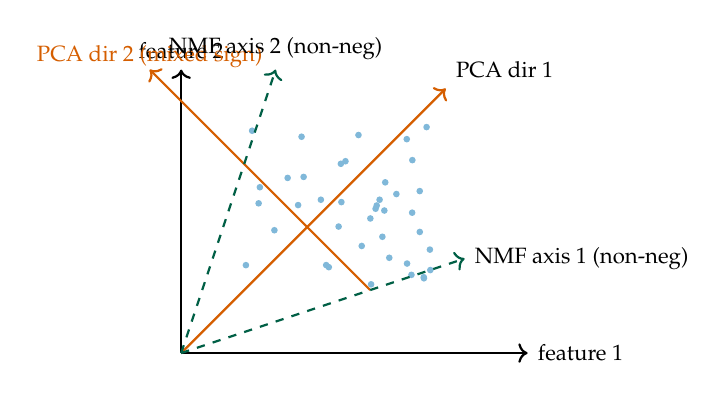
\begin{tikzpicture}[scale=0.8]
    \draw[->, thick] (0,0) -- (5.5, 0) node[right] {\footnotesize feature 1};
    \draw[->, thick] (0,0) -- (0, 4.5) node[above] {\footnotesize feature 2};

    \foreach \i in {1,...,40} {
        \pgfmathsetmacro{\x}{1 + 3*rnd}
        \pgfmathsetmacro{\y}{1 + 3*rnd}
        \fill[blue!50] (\x, \y) circle (1.5pt);
    }

    \draw[red, thick, ->] (0, 0) -- (4.2, 4.2) node[above right, black] {\footnotesize PCA dir 1};
    \draw[red, thick, ->] (3, 1) -- (-0.5, 4.5);
    \node[red] at (-0.5, 4.7) {\footnotesize PCA dir 2 (mixed sign)};

    \draw[green!60!black, thick, ->, dashed] (0, 0) -- (4.5, 1.5) node[right, black] {\footnotesize NMF axis 1 (non-neg)};
    \draw[green!60!black, thick, ->, dashed] (0, 0) -- (1.5, 4.5) node[above, black] {\footnotesize NMF axis 2 (non-neg)};
\end{tikzpicture}
\end{center}

\vspace{6pt}
\textbf{PCA} (red): orthogonal axes capturing maximum variance, but axis 2 has negative components.

\vspace{4pt}
\textbf{NMF} (green): non-orthogonal but non-negative axes. Each axis is a ``part'' that you \emph{add} to build the data.

\textcolor{red}{Different geometric prior, very different interpretation.}
\end{frame}

\begin{frame}
\frametitle{NMF: The Optimization Problem}

\textbf{Given:} non-negative matrix $\vY \geq 0$ of size $M \times N$.

\vspace{4pt}
\textbf{Find:} non-negative $\vU \in \R_{+}^{M \times K}$ and $\vV \in \R_{+}^{N \times K}$ such that $\vY \approx \vU \vV^\top$.

\vspace{8pt}
\textbf{Two common loss functions:}

\vspace{4pt}
\textbf{Squared loss}
\[
    \min_{\vU \geq 0,\, \vV \geq 0} \sum_{i,j} \bigl(Y_{ij} - \vu_i^\top \vv_j\bigr)^2
\]
penalizes squared distance.

\vspace{8pt}
\textbf{Generalized KL divergence (a.k.a.\ unnormalized KL)}
\[
    \min_{\vU \geq 0,\, \vV \geq 0} \sum_{i,j} Y_{ij} \log \frac{Y_{ij}}{\vu_i^\top \vv_j} - Y_{ij} + \vu_i^\top \vv_j
\]
penalizes ratio -- more appropriate for count data.

\vspace{4pt}
\textcolor{blue}{Train with multiplicative updates (Lee \& Seung, 2001) or projected gradient descent.}
\end{frame}

\begin{frame}
\frametitle{Faces: PCA vs NMF}

\textbf{Same dataset, two decompositions:}

\vspace{4pt}
\textbf{PCA} (eigenfaces):
\begin{itemize}
    \item Each basis face has both positive and negative pixels.
    \item Coefficients can be negative.
    \item Reconstructions look ``ghostly'' -- holistic faces.
    \item Few basis elements give a good reconstruction.
\end{itemize}

\vspace{6pt}
\textbf{NMF} (non-negative basis):
\begin{itemize}
    \item Each basis face is a localized ``part'' -- nose region, eye region, jaw.
    \item Coefficients are non-negative -- they say \emph{how much} of each part to use.
    \item Reconstructions assemble parts additively.
    \item Need more basis elements for the same reconstruction quality.
\end{itemize}

\vspace{6pt}
\textcolor{red}{Tradeoff: NMF is less compact but far easier to interpret.}
\end{frame}

\begin{frame}
\frametitle{Topic Modeling: NMF on Text}

\textbf{Setup:} build a document-by-word \emph{count} matrix $\vY \in \R_+^{M \times N}$.

\vspace{4pt}
$Y_{ij}$ = number of times word $j$ appears in document $i$.

\vspace{8pt}
\textbf{Apply NMF with $K$ topics:}
\begin{itemize}
    \item $\vU \in \R_{+}^{M \times K}$: how much of each topic appears in each document.
    \item $\vV \in \R_{+}^{N \times K}$: which words characterize each topic.
\end{itemize}

\vspace{8pt}
\textbf{Interpretation:}
\begin{itemize}
    \item Sort each column of $\vV$ by weight, top words define the topic.
    \item Sort each row of $\vU$ to see the document's topic mixture.
\end{itemize}

\vspace{6pt}
\textbf{LDA connection:} Latent Dirichlet Allocation is the probabilistic cousin of NMF -- same conceptual structure, different statistical assumptions.
\end{frame}

\begin{frame}
\frametitle{Econ Applications of NMF / LDA on Text}

\textbf{Three landmark papers:}

\vspace{6pt}
\begin{enumerate}
    \item \textbf{Hansen, McMahon, Prat (2018, QJE).}\\
    LDA on FOMC transcripts. Shows that committee deliberation patterns predict policy decisions and macro outcomes.

    \vspace{6pt}
    \item \textbf{Gentzkow, Shapiro, Taddy (2019, \emph{Econometrica}).}\\
    Text-as-data framework using bilinear / NMF-style decompositions. Recovers ideological positions of US politicians from speech.

    \vspace{6pt}
    \item \textbf{Bandiera, Prat, Hansen, Sadun (2020, JPE).}\\
    Topic models on CEO time-use diaries. Recovers two CEO ``types'' that predict firm performance.
\end{enumerate}

\vspace{8pt}
\textcolor{red}{Pattern:} reduce a high-dimensional, sparse, non-negative count matrix to a small set of interpretable factors. Then run regular econometrics on those factors.
\end{frame}

\begin{frame}
\frametitle{SVD/PCA vs NMF: Side-by-Side}

\renewcommand{\arraystretch}{1.3}
\begin{center}
{\small
\begin{tabular}{p{4cm} p{4.5cm} p{4.5cm}}
\toprule
& \textbf{SVD / PCA} & \textbf{NMF} \\
\midrule
Basis vectors & orthonormal, mixed sign & non-negative, non-orthogonal \\
Coefficients & any sign & non-negative \\
Geometric meaning & best rotation of axes & cone of additive parts \\
Interpretability & holistic, ghostly & parts-based, intuitive \\
Reconstruction quality & best at fixed $K$ & needs more components \\
Best for & Gaussian-like data & non-negative / count data \\
\bottomrule
\end{tabular}
}
\end{center}

\vspace{8pt}
\textcolor{blue}{Choose based on the data and the question.} For interpretability with non-negative data, NMF wins. For pure compression, SVD wins.
\end{frame}


% ============================================================
\section{Bridge to Deep Learning}
% ============================================================

\begin{transitionframe}
\begin{center}
{\Huge \textbf{Bridge to Deep Learning}}\\[10pt]
{\large What changes when we go non-linear?}
\end{center}
\end{transitionframe}

\begin{frame}
\frametitle{PCA Is a Linear Autoencoder}

\textbf{Encoder--decoder view:}
\[
    \vx \xrightarrow{\;\text{encode}\;} \vz = \vU^\top \vx \xrightarrow{\;\text{decode}\;} \hat{\vx} = \vU \vz
\]

\vspace{6pt}
$\vU$ is the same on both sides -- this is called \textbf{tied weights}.

\vspace{8pt}
\textbf{Loss:}
\[
    \min_{\vU} \sum_i \|\vx_i - \vU \vU^\top \vx_i\|^2
\]

\vspace{6pt}
\textbf{Solution:} the columns of $\vU$ are the top-$K$ left singular vectors. \emph{This is exactly PCA.}

\vspace{8pt}
\textbf{Generalization:} replace the linear encoder $\vU^\top$ with a deep network, the linear decoder $\vU$ with another deep network, and untie the weights. You get a \textbf{deep autoencoder}.

\vspace{4pt}
\textcolor{red}{The benefit:} the bottleneck $\vz$ can capture non-linear manifolds (faces with expression, lighting, pose) that PCA can't.
\end{frame}

\begin{frame}[fragile]
\frametitle{Embedding Layers Are Matrix Factorization}

\textbf{In PyTorch:}
\begin{lstlisting}
emb = nn.Embedding(num_users, K)
u_i = emb(user_id)  # K-dim vector
\end{lstlisting}

\vspace{6pt}
\textbf{What this is doing:} \texttt{emb.weight} is a $\text{num\_users} \times K$ matrix. \texttt{emb(user\_id)} returns row \texttt{user\_id}. That's the user vector $\vu_i$ from collaborative filtering.

\vspace{6pt}
\textbf{Two embeddings + dot product = matrix factorization.}

\vspace{8pt}
\textbf{Where it matters:}
\begin{itemize}
    \item Recommender systems (user $\times$ item).
    \item Word embeddings (word $\times$ context word).
    \item Knowledge graph embeddings (entity $\times$ relation $\times$ entity).
    \item Two-tower retrieval models (query $\times$ document).
\end{itemize}

\vspace{4pt}
\textcolor{red}{Whenever you see an embedding layer, you're looking at the $\vU$ from this lecture.}
\end{frame}

\begin{frame}
\frametitle{Word2vec Is Implicit Matrix Factorization}

\textbf{Skip-gram with negative sampling} (Mikolov et al., 2013):
\begin{itemize}
    \item Slide a window over text.
    \item For each center word $w$ and context word $c$ in the window: predict ``$w$ and $c$ co-occur''.
    \item For randomly drawn negative pairs: predict ``they don't''.
\end{itemize}

\vspace{8pt}
\textbf{Levy \& Goldberg (NIPS 2014) theorem:} this objective implicitly factorizes the matrix
\[
    M_{wc} = \mathrm{PMI}(w, c) - \log k
\]
where PMI is pointwise mutual information and $k$ is the negative-sampling rate.

\vspace{8pt}
\textcolor{blue}{Word2vec = SVD of the shifted PMI matrix.}

\vspace{4pt}
\textbf{Implications:}
\begin{itemize}
    \item Word embeddings are not magic -- they are matrix factorization in disguise.
    \item ``King $-$ man $+$ woman $\approx$ queen'' is exactly a low-rank linear-algebra property.
\end{itemize}
\end{frame}

\begin{frame}
\frametitle{What We've Built}

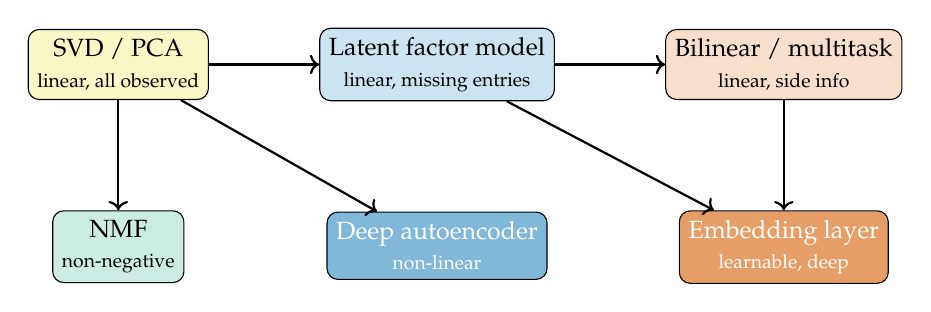
\begin{tikzpicture}[node distance=1.4cm, every node/.style={draw, rounded corners, align=center, font=\small}]
    \node (svd) [fill=yellow!30] {SVD / PCA \\ \scriptsize linear, all observed};
    \node (lfm) [right=of svd, fill=blue!20] {Latent factor model \\ \scriptsize linear, missing entries};
    \node (mtl) [right=of lfm, fill=red!20] {Bilinear / multitask \\ \scriptsize linear, side info};
    \node (nmf) [below=of svd, fill=green!20] {NMF \\ \scriptsize non-negative};
    \node (ae) [below=of lfm, fill=blue!50, text=white] {Deep autoencoder \\ \scriptsize non-linear};
    \node (emb) [below=of mtl, fill=red!60, text=white] {Embedding layer \\ \scriptsize learnable, deep};

    \draw[->, thick] (svd) -- (lfm);
    \draw[->, thick] (lfm) -- (mtl);
    \draw[->, thick] (svd) -- (nmf);
    \draw[->, thick] (svd) -- (ae);
    \draw[->, thick] (lfm) -- (emb);
    \draw[->, thick] (mtl) -- (emb);
\end{tikzpicture}

\vspace{8pt}
\textbf{One thread runs through everything:} learn a low-dimensional representation that captures the structure of the data.

\vspace{4pt}
\textcolor{red}{Linear bottleneck $\to$ non-linear bottleneck = the move from classical ML to deep learning.}
\end{frame}


% ============================================================
\section{Summary and Next Steps}
% ============================================================

\begin{transitionframe}
\begin{center}
{\Huge \textbf{Summary \& Next Steps}}
\end{center}
\end{transitionframe}

\begin{frame}
\frametitle{Today's Big Ideas}

\begin{enumerate}
    \item \textbf{SVD is the master decomposition.} Best low-rank approximation in Frobenius norm; the foundation of PCA, eigenfaces, and everything that follows.

    \vspace{4pt}
    \item \textbf{Trace norm is the convex envelope of rank.} Replaces a discrete penalty with a smooth one -- the matrix analogue of L1.

    \vspace{4pt}
    \item \textbf{Latent factor models} solve matrix completion with $\vY \approx \vU \vV^\top$ via Frobenius regularization on the factors.

    \vspace{4pt}
    \item \textbf{Panel data view.} Same model as Bai (2009) interactive fixed effects; matrix completion of treated cells gives causal counterfactuals (Athey et al.\ 2021).

    \vspace{4pt}
    \item \textbf{NMF} replaces orthogonality with non-negativity. Yields parts-based, interpretable bases. Core technology for topic modeling.

    \vspace{4pt}
    \item \textbf{Bridge to DL.} Embedding layers, autoencoders, and word2vec are all matrix factorization with extra moving parts.
\end{enumerate}
\end{frame}

\begin{frame}
\frametitle{Practical Recipes}

\textbf{When to use what:}
\begin{itemize}
    \item Need to compress dense, mixed-sign data $\to$ \textbf{PCA / SVD}.
    \item Have a sparse user-by-item matrix $\to$ \textbf{latent factor models with ALS}.
    \item Causal inference with panel data and missing potential outcomes $\to$ \textbf{matrix completion} (\texttt{gsynth}, \texttt{pysyncon}).
    \item Topic modeling or non-negative parts $\to$ \textbf{NMF} (\texttt{sklearn.decomposition.NMF}).
    \item Deep features and large-scale learning $\to$ \textbf{embedding layers + neural net}.
\end{itemize}

\vspace{8pt}
\textbf{Common bug:} trying to apply SVD to a matrix with missing entries. SVD requires every cell -- if you have missing data, use the latent factor formulation with the indicator $\omega_{ij}$, not raw SVD.

\vspace{6pt}
\textbf{Common bug:} forgetting to standardize before PCA. PCA without centering puts the first component in the direction of the mean, not the maximum variance.
\end{frame}

\begin{frame}
\frametitle{Next Lecture: Embeddings and Attention}

\textbf{Lecture 7:}
\begin{itemize}
    \item Embedding learning beyond linear factor models.
    \item Word2vec, item2vec, sentence embeddings.
    \item The attention mechanism: queries, keys, values.
    \item Self-attention as content-aware embedding lookup.
    \item Foundation for Transformers (Lecture 8).
\end{itemize}

\vspace{8pt}
\textbf{The big picture:}
\begin{center}
\textit{SVD $\to$ Latent factors $\to$ Embeddings $\to$ Attention $\to$ Transformers}
\end{center}

\vspace{6pt}
\textbf{Recommended reading before next class:}
\begin{itemize}
    \item Mikolov et al. (2013), \emph{Distributed representations of words and phrases}.
    \item Levy \& Goldberg (2014), \emph{Neural word embedding as implicit matrix factorization}.
    \item Athey et al.\ (2021) intro section, \emph{Matrix completion methods for causal panel data}.
\end{itemize}

\vspace{6pt}
\begin{center}
\Large \textcolor{blue}{\textbf{Questions?}}
\end{center}
\end{frame}

\begin{frame}
\frametitle{References}

\footnotesize
\begin{itemize}
    \item Eckart, C., \& Young, G. (1936). The approximation of one matrix by another of lower rank. \textit{Psychometrika}, 1(3).
    \item Lee, D. D., \& Seung, H. S. (1999). Learning the parts of objects by non-negative matrix factorization. \textit{Nature}, 401.
    \item Lee, D. D., \& Seung, H. S. (2001). Algorithms for non-negative matrix factorization. \textit{NIPS}.
    \item Koren, Y., Bell, R., \& Volinsky, C. (2009). Matrix factorization techniques for recommender systems. \textit{IEEE Computer}, 42(8).
    \item Bai, J. (2009). Panel data models with interactive fixed effects. \textit{Econometrica}, 77(4).
    \item Athey, S., Bayati, M., Doudchenko, N., Imbens, G., \& Khosravi, K. (2021). Matrix completion methods for causal panel data models. \textit{JASA}, 116(536).
    \item Xu, Y. (2017). Generalized synthetic control method. \textit{Political Analysis}, 25(1).
    \item Mikolov, T., Sutskever, I., Chen, K., Corrado, G., \& Dean, J. (2013). Distributed representations of words and phrases. \textit{NIPS}.
    \item Levy, O., \& Goldberg, Y. (2014). Neural word embedding as implicit matrix factorization. \textit{NIPS}.
    \item Hansen, S., McMahon, M., \& Prat, A. (2018). Transparency and deliberation within the FOMC. \textit{QJE}, 133(2).
    \item Gentzkow, M., Kelly, B., \& Taddy, M. (2019). Text as data. \textit{Journal of Economic Literature}, 57(3).
    \item Bandiera, O., Prat, A., Hansen, S., \& Sadun, R. (2020). CEO behavior and firm performance. \textit{JPE}, 128(4).
\end{itemize}
\end{frame}


\end{document}
